% !TEX root = ../paper.tex
\section{Experiment} \label{sec:experiment}
% Intro
In order to compare the different techniques to each other we conducted an experiment in which each participant would perform the techniques in a controlled environment.
There are two parts to this experiment because after we finished the first experiment we realized that before we could say anything about accuracy in pixels we would have to tell people to aim and be as precise as they possibly can.
Not having told our first 51 participants to aim and be precise we did the experiment again with a few changes

% Explaining the difference between the two parts
In the first part of the experiment, participants are instructed to hit the target on the screen and a yellow background color is shown on the cell where the blue pointer is \Cref{fig:target}.
This background color snaps the pointer to the grid making the target appear selected.
For the second part of the experiment, the targets on the large display would have a cross in the middle and the yellow snap-to-grid background was removed \Cref{fig:accuracy}.
In the second part participants were instructed to be as precise as possible and hit the center of the target.
These are the only differences between the two parts of the experiment.
\begin{figure}[H]
\centering
\subfloat[]{\includegraphics[width = 0.13\columnwidth]{images/target.pdf}\label{fig:target}}
\hspace{0.05\columnwidth}
\subfloat[]{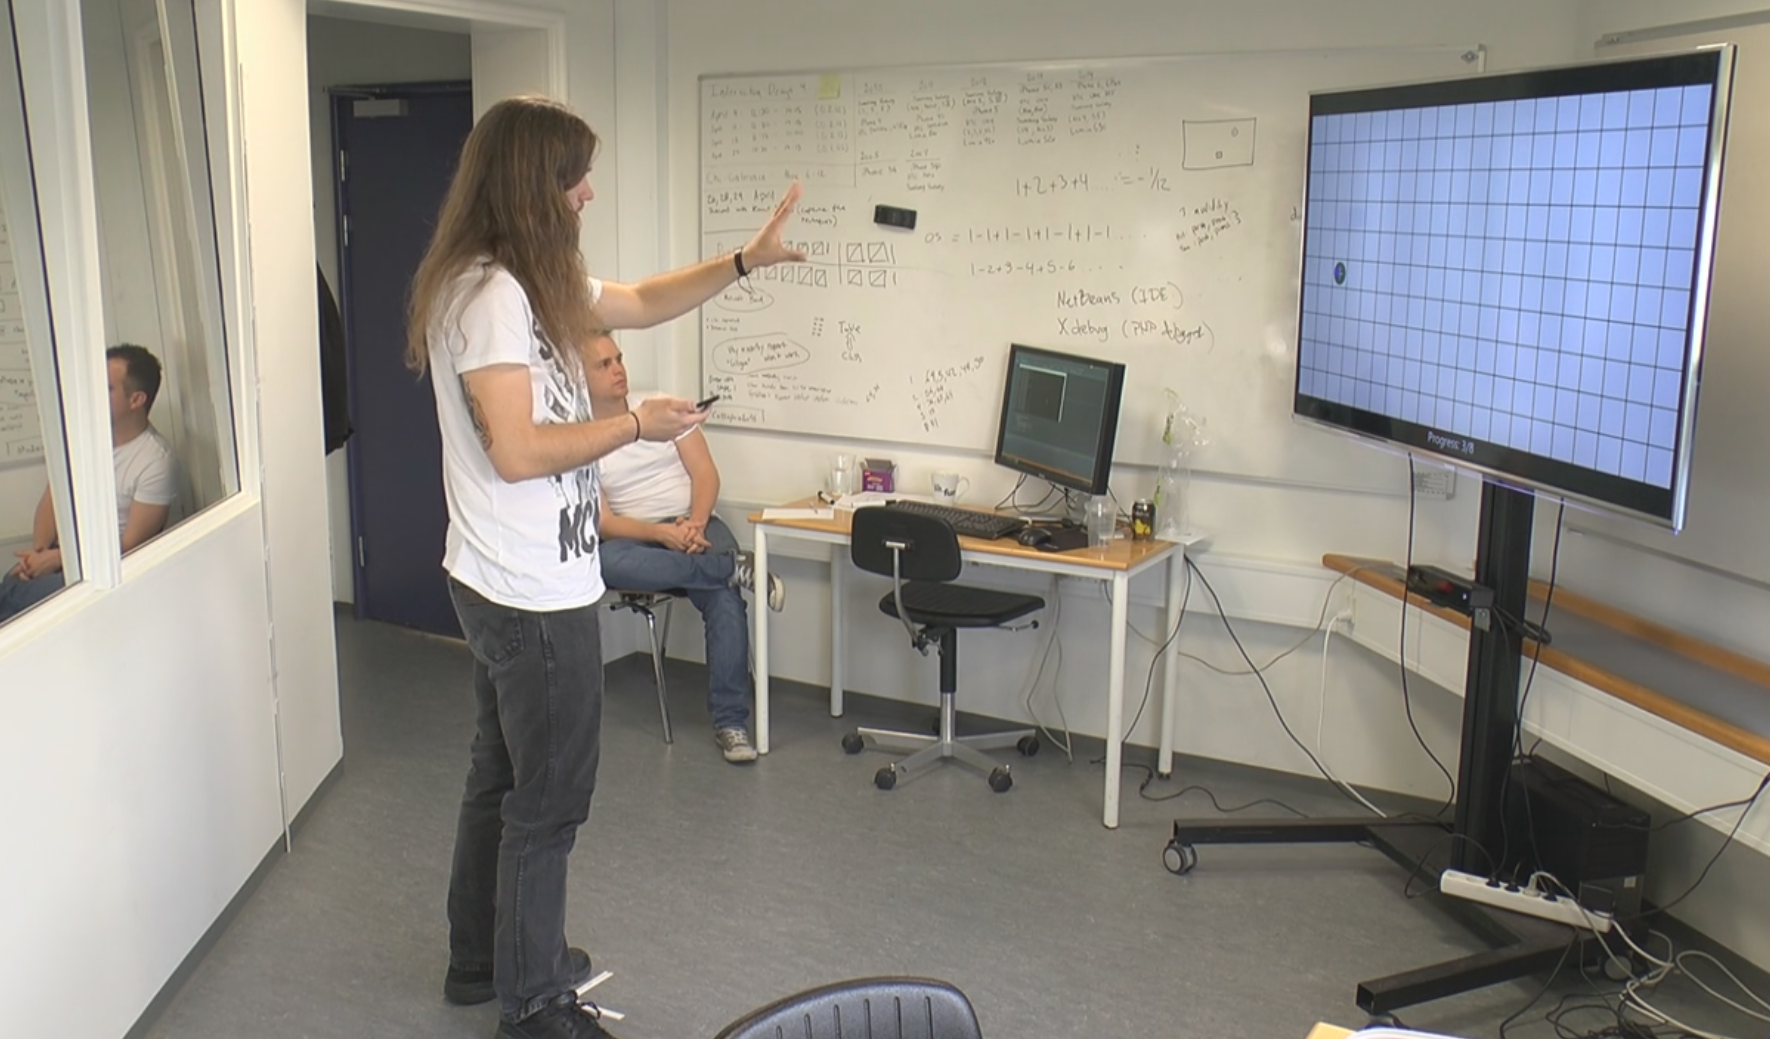
\includegraphics[width = 0.13\columnwidth]{images/accuracy.pdf}\label{fig:accuracy}}
\caption{\protect\subref{fig:target} The targets in the first part of the experiment. \protect\subref{fig:accuracy} The targets in the second part of the experiment.}
\end{figure}

\subsection{Experimental Setup} \label{sec:setup}
% The setup and the hardware used in the experiment
The experiment was conducted in the usability lab where we had setup a large 65'' screen (1920$\times$1080 pixels) and a smaller 42'' screen (1024$\times$768 pixels) as seen in \Cref{fig:setupPhoto}.
A Microsoft Kinect v2 was mounted below the large display (81 cm above the floor) and we marked the floor with a cross (200 cm from the Kinect) where participants were told to stand.
The phone we used in this experiment was a Samsung Galaxy S2 (4.3'' screen).
The setup is illustrated in \Cref{fig:setup}.

\begin{figure}[H]
\subfloat[]{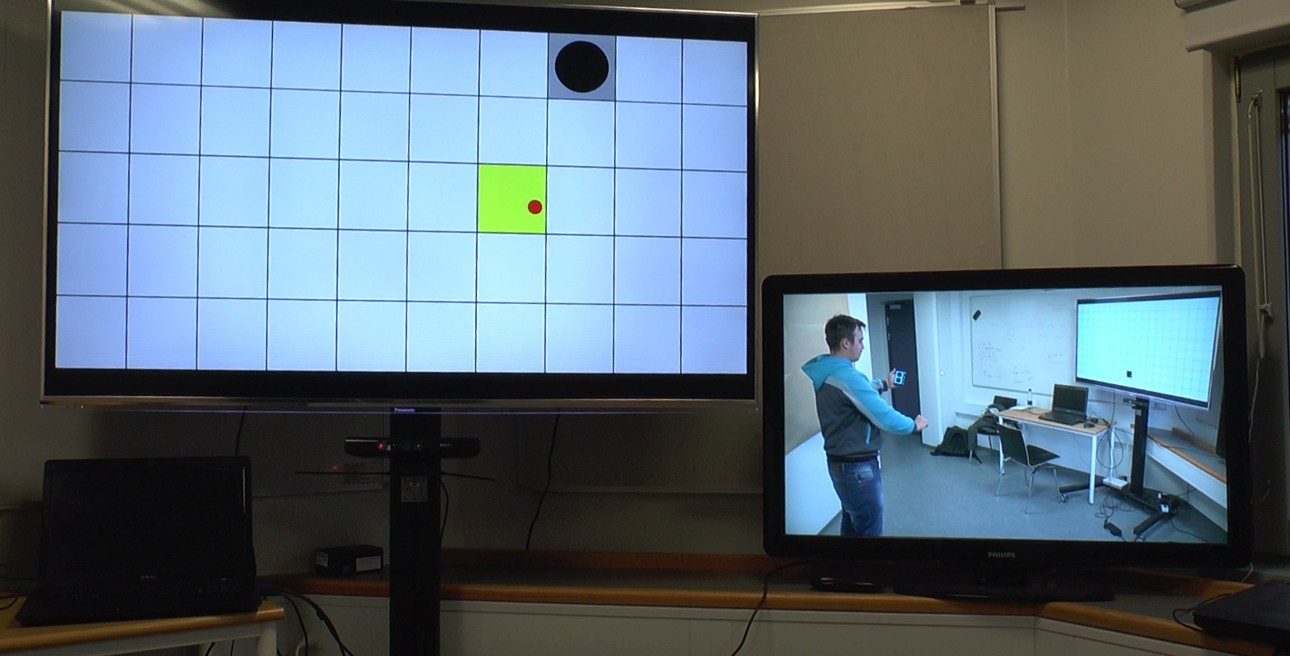
\includegraphics[width = 0.6\columnwidth]{images/setup.jpg}\label{fig:setupPhoto}}
\subfloat[]{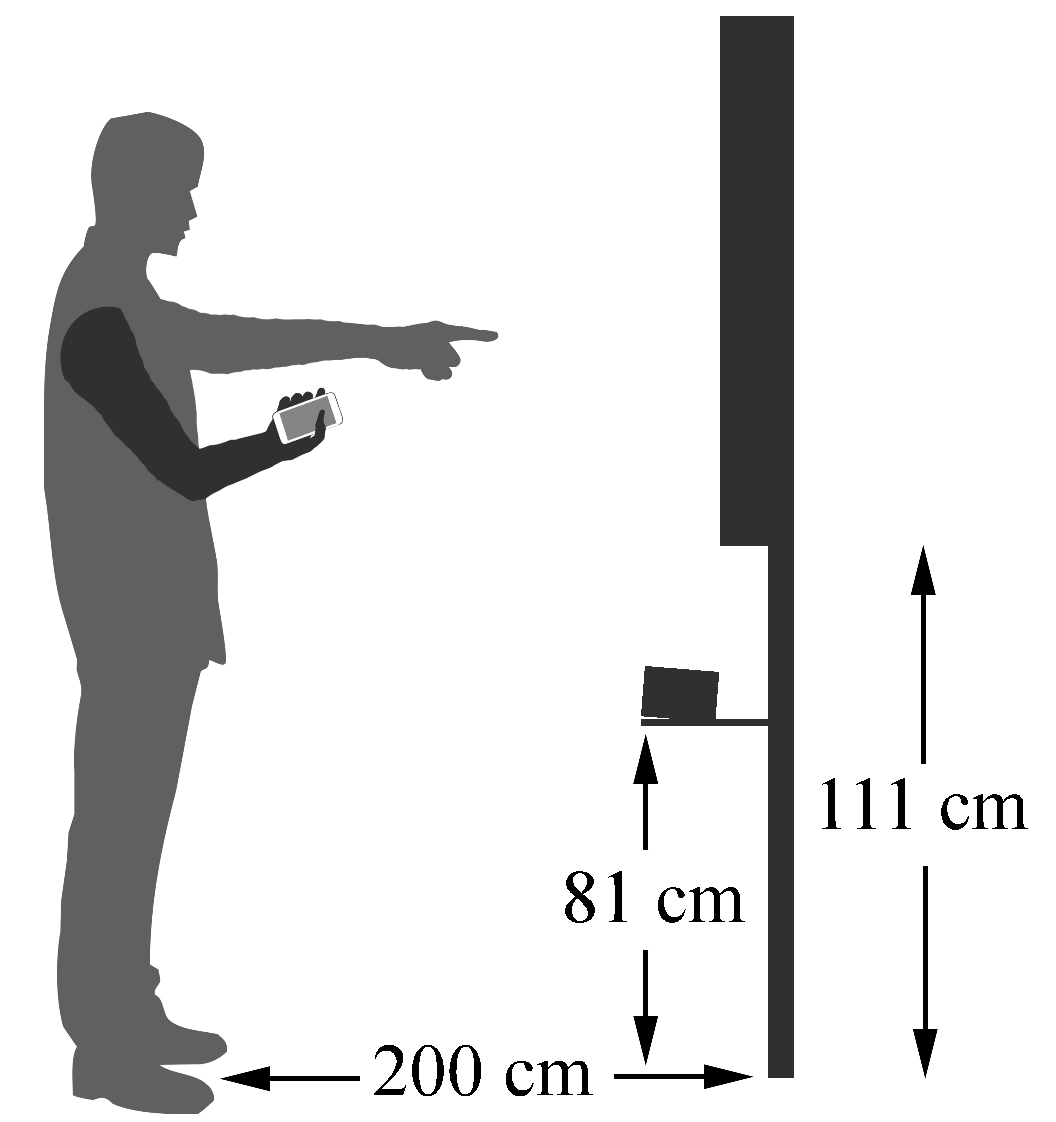
\includegraphics[width = 0.37\columnwidth]{images/setup.pdf}\label{fig:setup}}
\caption{\protect\subref{fig:setupPhoto} the setup in the usability lab. \protect\subref{fig:setup} illustrates the setup and distance between participant and screen, floor and Kinect, and floor and the bottom of the large display.}
\end{figure}

\subsubsection{Design} \label{}
% (explain practice targets, targets, grid, before procedure and task section)
% Also, explain sequences and the different distances between targets
A within-group design was used for the experiment and each participant would use all 8 techniques once during the experiment.
We have 2 different target sizes and 8 techniques (push = 4, pull = 4) as the independent variables.
For each technique there are a total of 18 targets and 3 practice targets at the beginning of each technique. 
Practice targets allows the participants to get familiar with the technique before we start collecting data for a technique.
The 2 different sizes of targets are 9 small and 9 large targets, which are placed in a square grid cell.
We use a grid to give the yellow highlighted ``snap-to-grid'' background meaning (see \cref{fig:target}).
The size of the small grid is 10$\times$5 cells where each cell is 61 pixels (7.3 cm) wide and the size of the large grid is 20$\times$10 cells where each cell is 122 pixels (14.6 cm) wide.
A target appears in a cell in a predetermined sequence to make sure that all participants are given same distances between targets and the sequences are then randomly assigned to a technique for each participant for randomization.
The order in which the participants are given a technique is randomized to minimize the learning effect.
For both \target and \accuracy 51\% of the participants started with \push techniques and 49\% started with \pull techniques.
For the \target 27\% of the participants started the test with \grab, 21\% with \swipe, 25\% with \throw, and 27\% with \tilt.
Similarly, for the \accuracy 22\% of the participants started the test with \grab, 27\% with \swipe, 24\% with \throw, and 27\% with \tilt.
For \target the total amount of attempts collected were 2 target sizes $\times$ 8 techniques $\times$ 9 repetitions $\times$ 51 participants = 7344 attempts and for \accuracy the total is 2 target sizes $\times$ 8 techniques $\times$ 9 repetitions $\times$ 33 participants = 4752 attempts.

\subsection{Task \& Procedure} \label{sec:procedure}
Before a participant starts the experiment, the general purpose of the study is explained to the participant and we tell them what is going to happen.
Then a demonstration video of a technique is shown on the large screen and after watching the video it plays in a loop on the small screen.
The participant is then presented with the grid and one target after another will appear in the grid until the participant has attempted to hit all targets.
After completing one technique the remaining techniques follow with the same procedure as the first until all 8 techniques have been performed.
When a participant has done all the techniques we give them a short demographic questionnaire including age, height, gender, current phone, year of first smartphone, and if they have had prior experience with systems like the Nintendo Wii or the Microsoft Kinect.
The average time for completing the experiment per participant was \todo[inline]{Insert the avg. time here}

\begin{figure}[H]
\subfloat[\push]{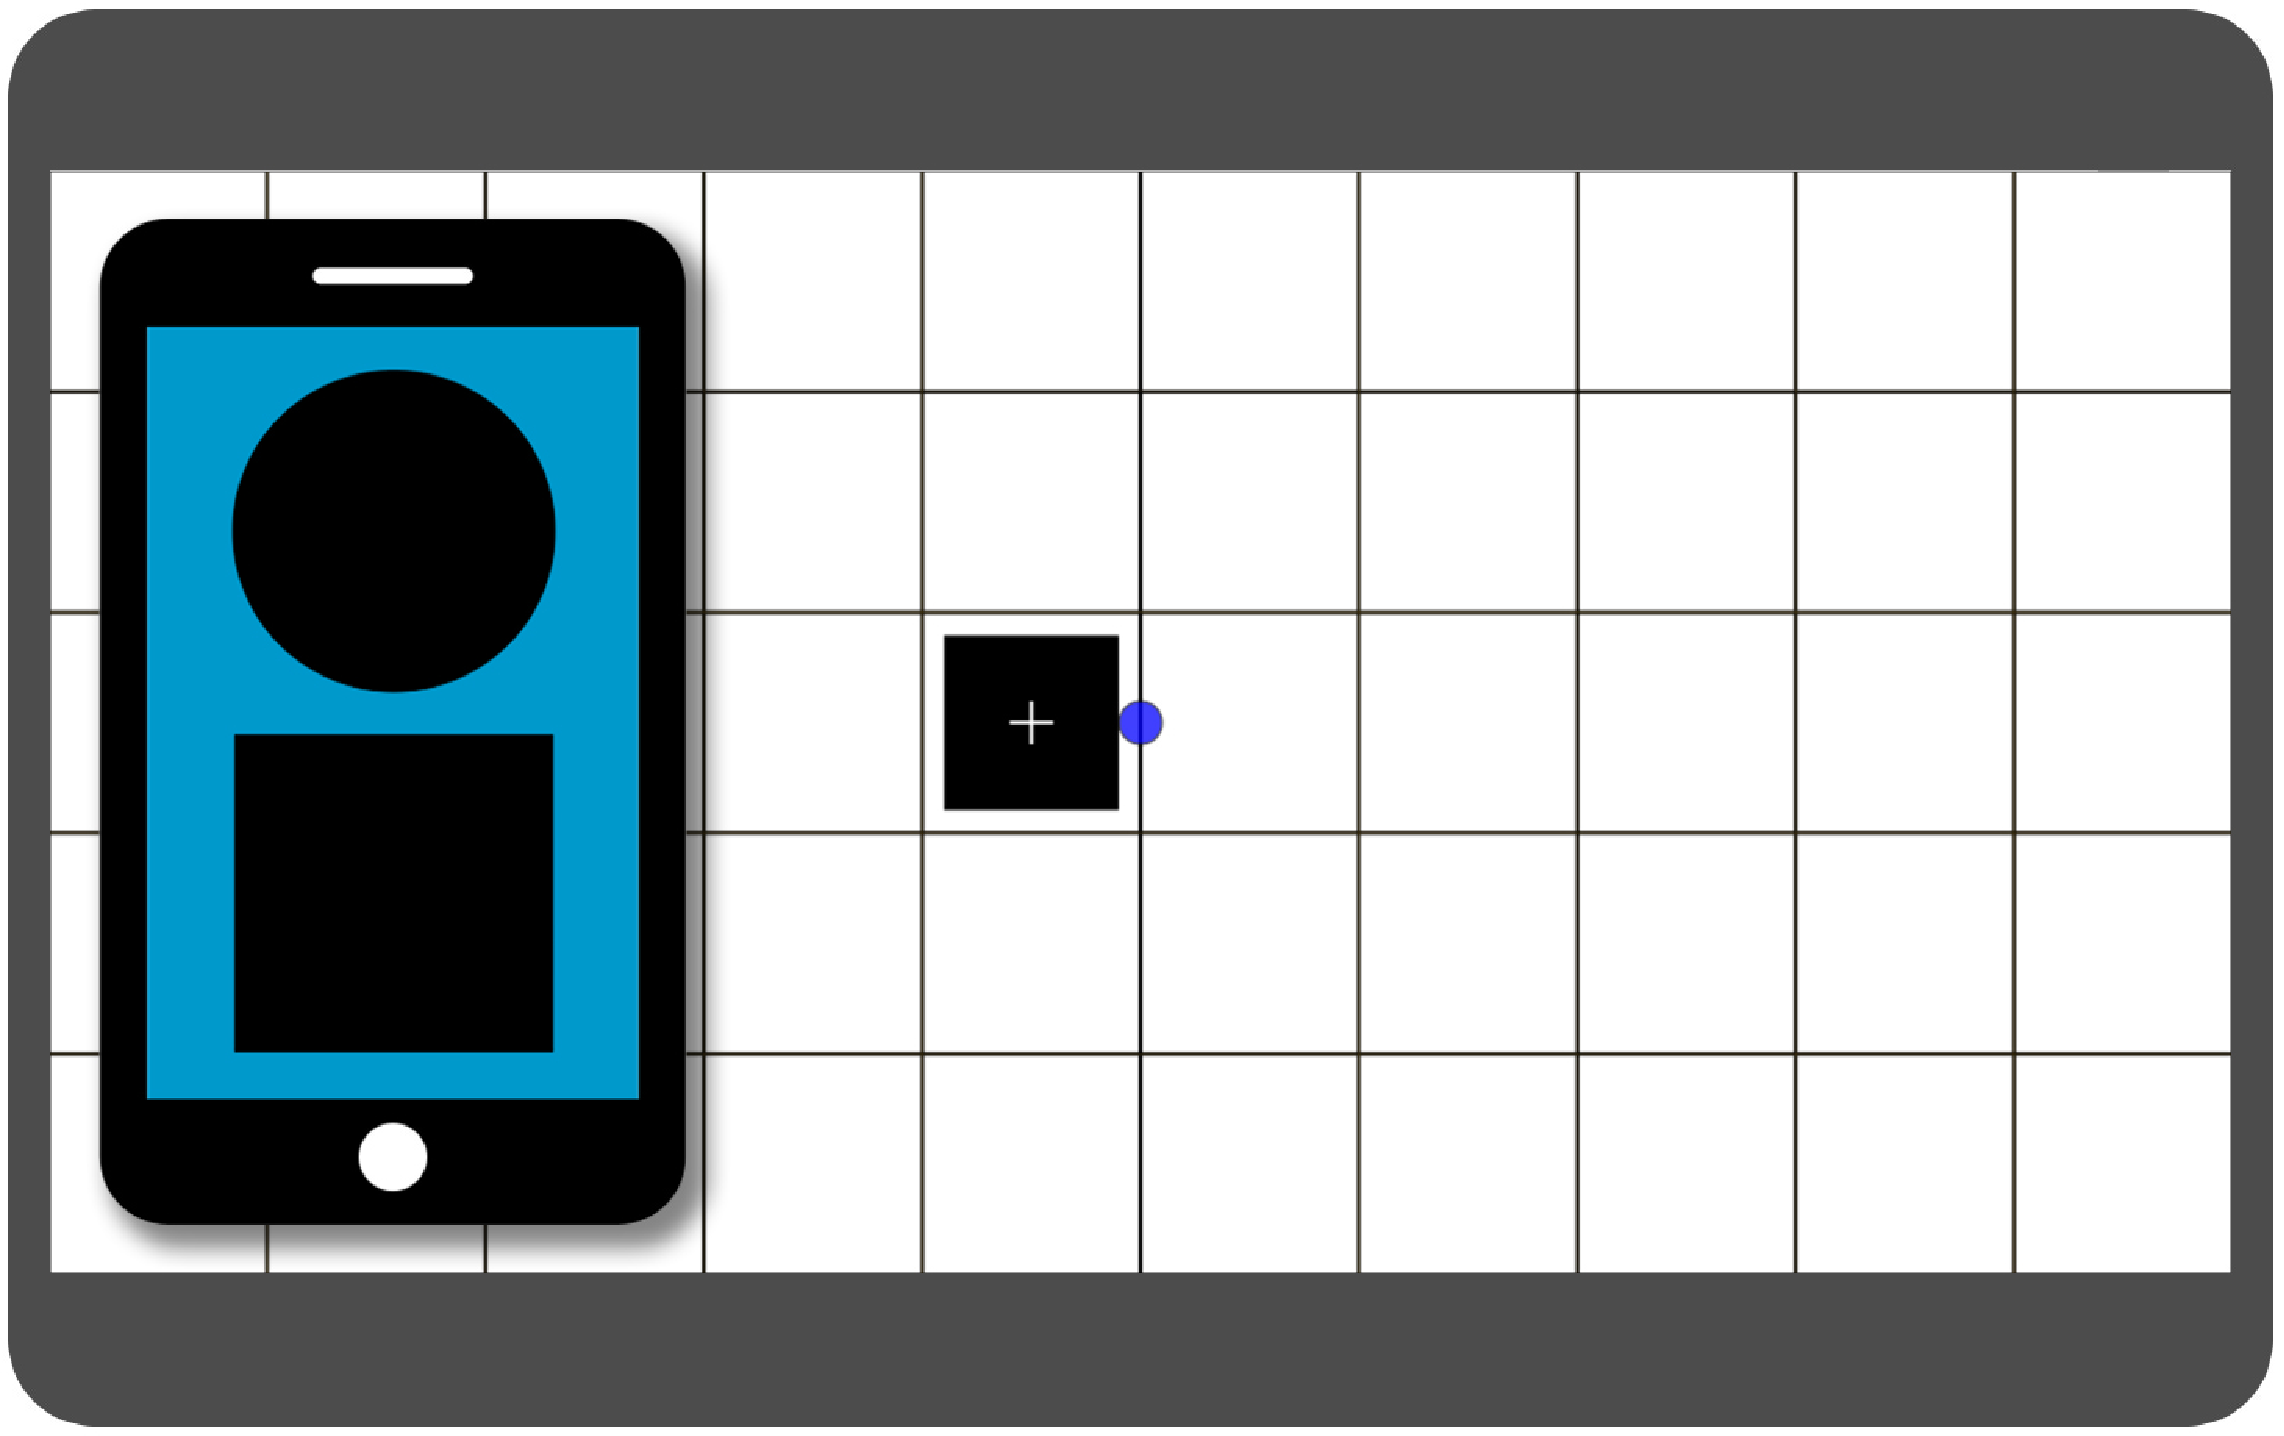
\includegraphics[width = 0.49\columnwidth]{images/pushScreen.pdf}\label{fig:pushScreen}}
\hspace{0.01\columnwidth}
\subfloat[\pull]{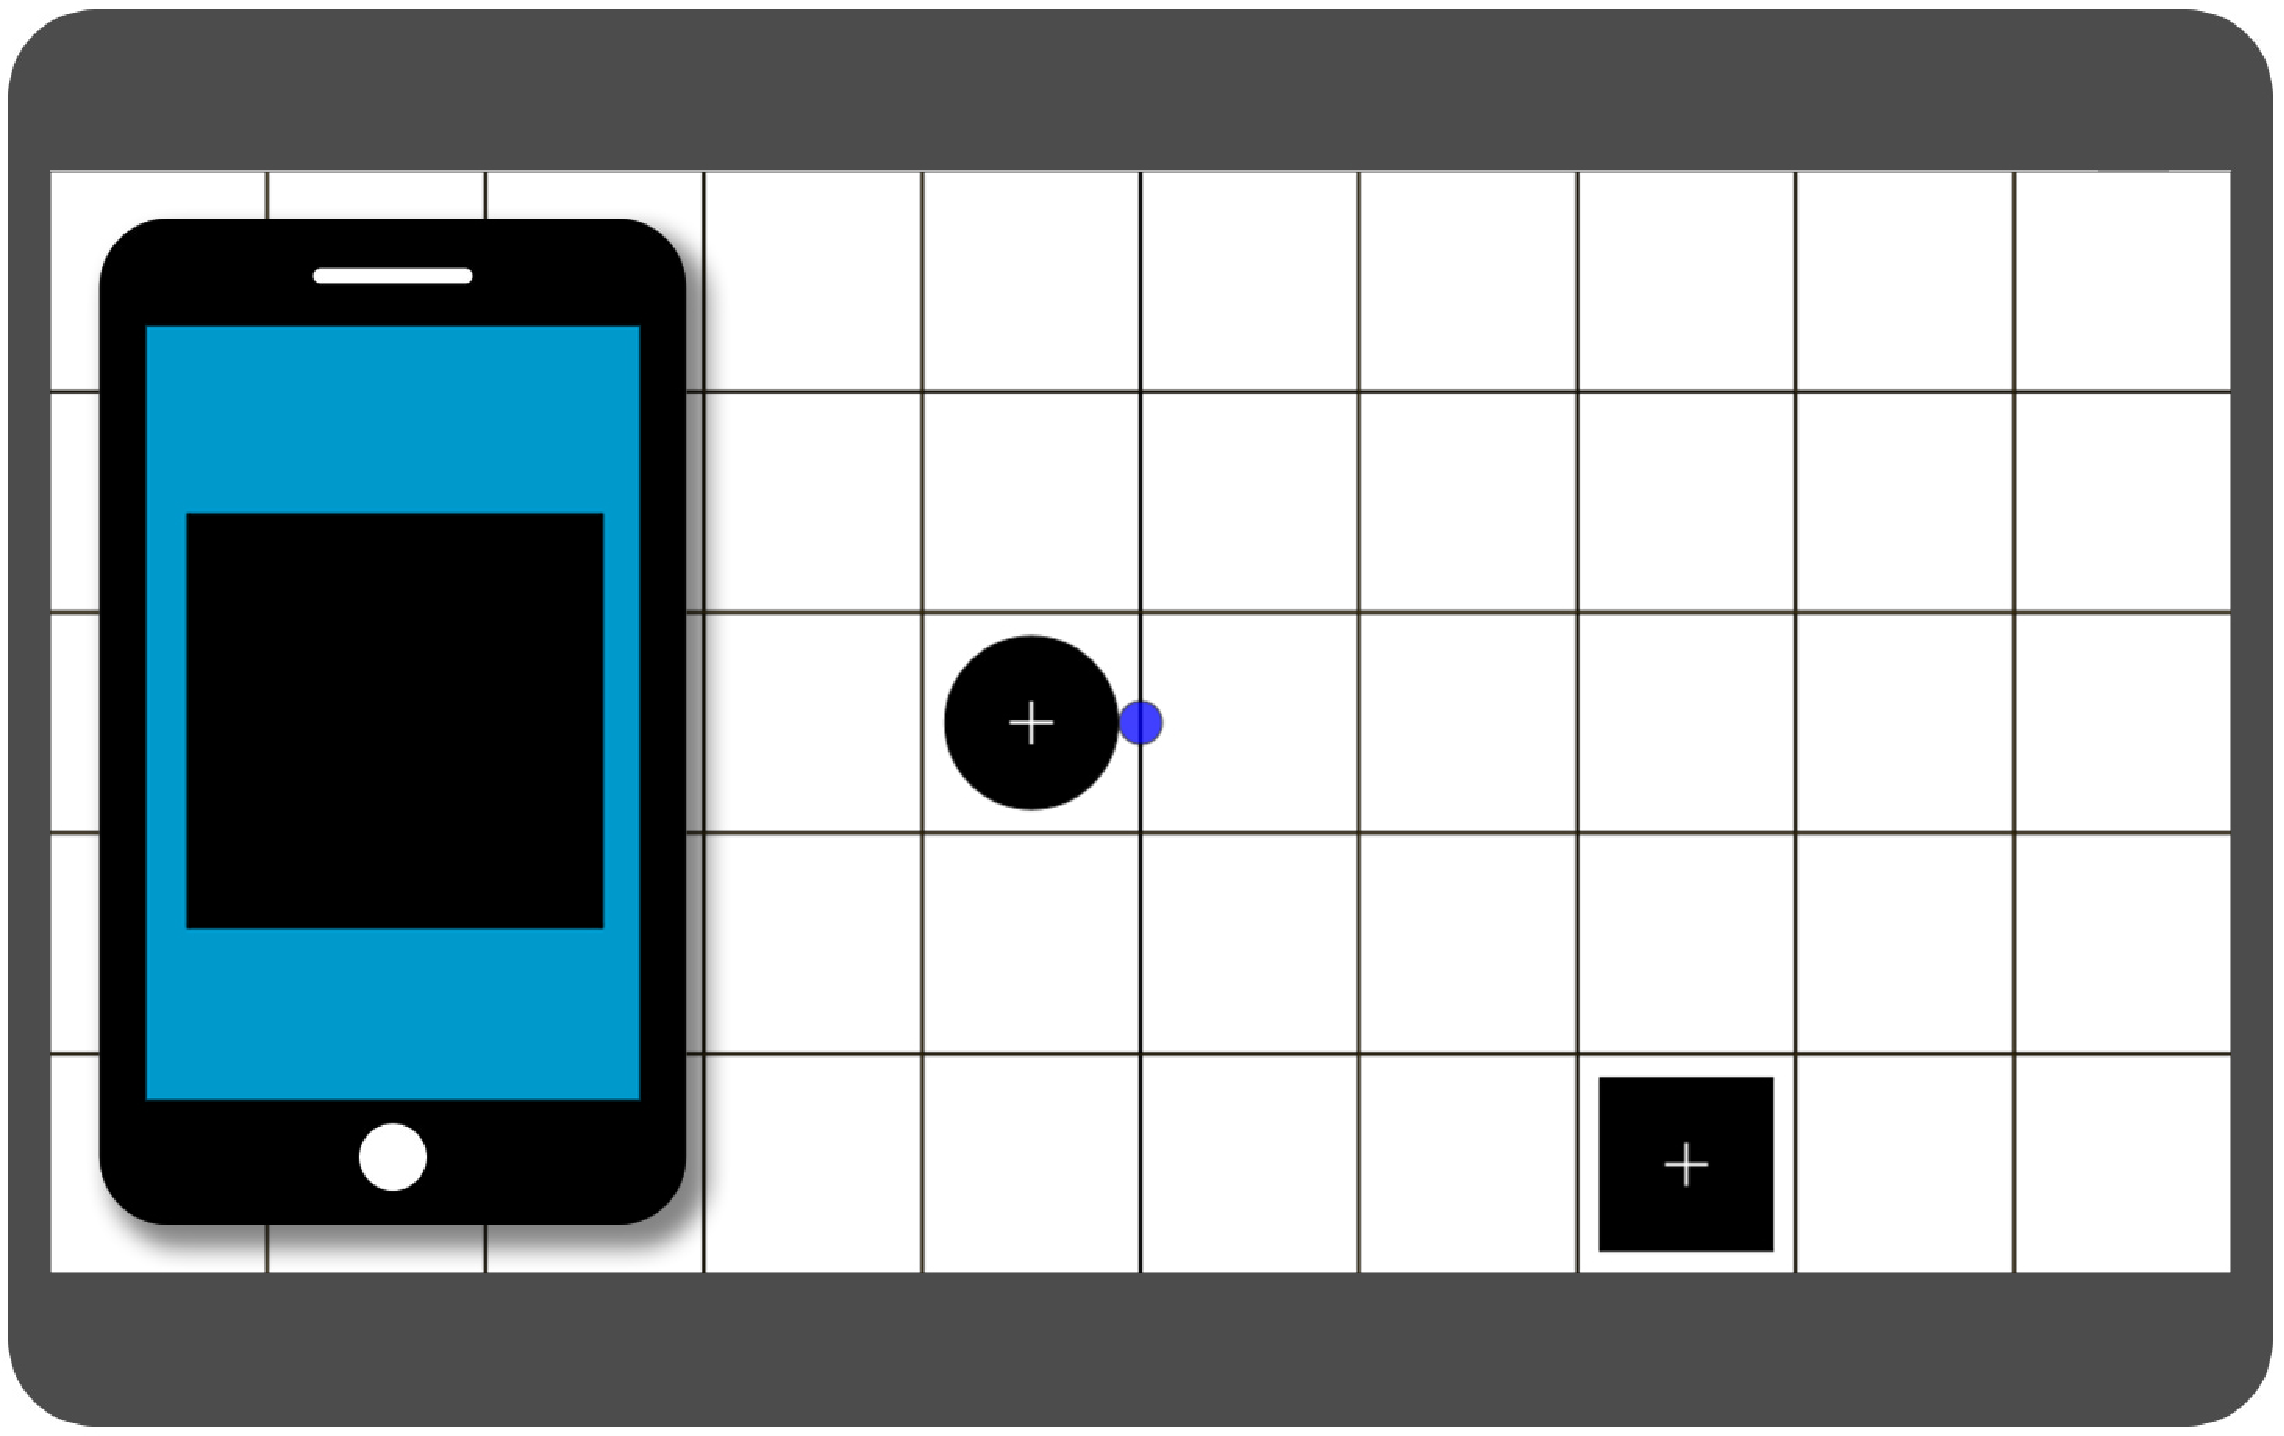
\includegraphics[width = 0.49\columnwidth]{images/pullScreen.pdf}\label{fig:pullScreen}}
\caption{The screens on both the large display and the phone for the \accuracy.}
\end{figure}